% !TeX root = ../main.tex
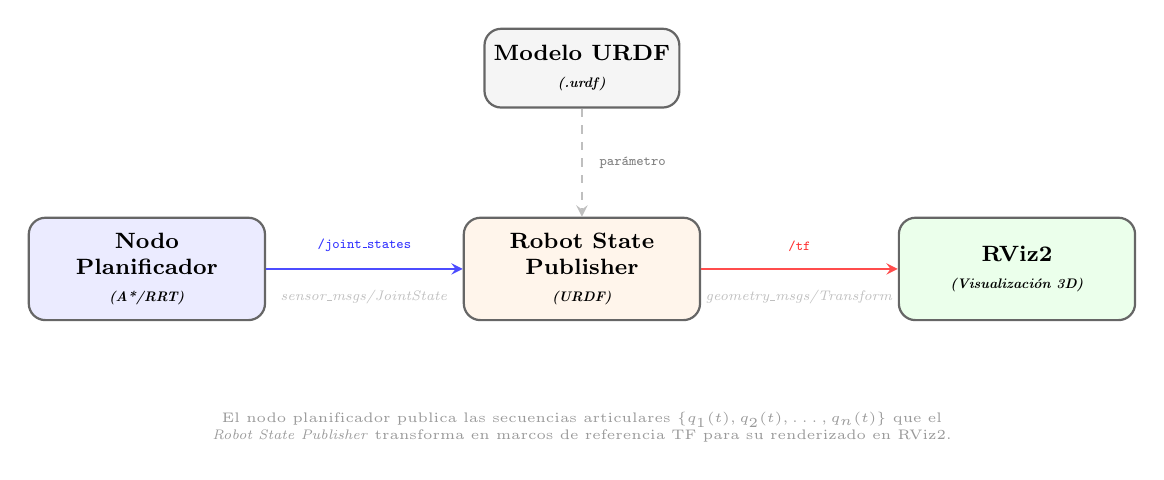
\begin{tikzpicture}[>=stealth, scale=0.85, every node/.style={font=\small},
    % Estilos de nodos
    rosnode/.style={
        draw=black!60, thick, rounded corners=6pt,
        fill=white, minimum width=3.0cm, minimum height=1.3cm,
        font=\footnotesize\bfseries, align=center
    },
    rostopic/.style={
        font=\tiny\ttfamily, fill=white, inner sep=2pt
    }
]

% =============================================
% NODOS ROS2
% =============================================

% Nodo Planificador (izquierda)
\node[rosnode, fill=blue!8] (planner) at (-6.5, 0) 
    {Nodo\\Planificador\\{\tiny\textit{(A*/RRT)}}};

% Robot State Publisher (centro)
\node[rosnode, fill=orange!8] (rsp) at (0, 0) 
    {Robot State\\Publisher\\{\tiny\textit{(URDF)}}};

% RViz2 (derecha)
\node[rosnode, fill=green!8] (rviz) at (6.5, 0) 
    {RViz2\\{\tiny\textit{(Visualización 3D)}}};

% Nodo URDF/modelo (arriba del RSP)
\node[rosnode, fill=gray!8, minimum width=2.4cm, minimum height=1cm] (urdf) at (0, 3) 
    {Modelo URDF\\{\tiny\textit{(.urdf)}}};

% =============================================
% CONEXIONES (Tópicos)
% =============================================

% Planificador → RSP via /joint_states
\draw[->, thick, blue!70] (planner.east) -- (rsp.west)
    node[rostopic, midway, above=4pt, text=blue!80] {/joint\_states}
    node[midway, below=4pt, font=\tiny, gray!50] {\textit{sensor\_msgs/JointState}};

% RSP → RViz2 via /tf
\draw[->, thick, red!70] (rsp.east) -- (rviz.west)
    node[rostopic, midway, above=4pt, text=red!80] {/tf}
    node[midway, below=4pt, font=\tiny, gray!50] {\textit{geometry\_msgs/Transform}};

% URDF → RSP (parámetro)
\draw[->, thick, gray!50, dashed] (urdf.south) -- (rsp.north)
    node[rostopic, midway, right=4pt, text=black!50] {parámetro};

% =============================================
% NOTA DESCRIPTIVA
% =============================================
\node[anchor=north, font=\tiny, text=black!40, text width=12cm, align=center] at (0, -2.0) 
    {El nodo planificador publica las secuencias articulares $\{q_1(t), q_2(t), \dots, q_n(t)\}$ que el \textit{Robot State Publisher} transforma en marcos de referencia TF para su renderizado en RViz2.};

\end{tikzpicture}
